\documentclass[12pt]{article}

\usepackage{graphicx}% Include figure files
\usepackage{dcolumn}% Align table columns on decimal point

% Use Arial font %
\usepackage{helvet}
\renewcommand{\familydefault}{\sfdefault} 

% Default margins and paper properties %
\usepackage[a4, portrait, margin=0.6in]{geometry}

\definecolor{black}{HTML}{000000}

\begin{document}
	\title{Hypothesis plots summary} % Force line breaks with \\
	\author{1666957, Gustavo Espinal Lugo}
	\date{\today} % It is always \today, today, %  but any date may be explicitly specified

	\maketitle
	%\tableofcontents
	
	\section*{Plots and corresponding metadata}
	Number of data points used: 1000, mean expected W mass: 80.36010913 [GeV/c^2], mean hypothesis masses: [79. 80. 81. 82. 83.] [GeV/c^2], mass width: 2.07041274 [GeV/c^2], chi_square value of hypothesis fit: 0.00029114840214308296\\
	Absolute path to figure: /home/physics/phuxdp/Desktop/WBosonProject/templates/plots/muPT_80.36010913_2.07041274_between_79_and_83.png\\
	Next lines are the data of the shown histograms (if needed): \\
	All quantities: 	1000, 80.36010913, [79. 80. 81. 82. 83.], 2.07041274, 0.00029114840214308296\\
	X_energ_vls = [0.6, 1.7999999999999998, 3.0, 4.199999999999999, 5.4, 6.6, 7.8, 9.0, 10.2, 11.399999999999999, 12.6, 13.799999999999999, 15.0, 16.2, 17.4, 18.6, 19.799999999999997, 21.0, 22.2, 23.4, 24.6, 25.799999999999997, 27.0, 28.199999999999996, 29.4, 30.6, 31.799999999999997, 33.0, 34.2, 35.4, 36.599999999999994, 37.8, 39.0, 40.2, 41.4, 42.599999999999994, 43.8, 45.0, 46.2, 47.4, 48.599999999999994, 49.8, 51.0, 52.2, 53.4, 54.599999999999994, 55.8, 57.0, 58.199999999999996, 59.4, 60.599999999999994, 61.8, 63.0, 64.19999999999999, 65.4, 66.6, 67.8, 69.0, 70.19999999999999, 71.4, 72.6, 73.8, 75.0, 76.19999999999999, 77.4, 78.6, 79.8, 81.0, 82.19999999999999, 83.4, 84.6, 85.8, 87.0, 88.19999999999999, 89.4, 90.6, 91.8, 93.0, 94.19999999999999, 95.4, 96.6, 97.8, 99.0, 100.19999999999999, 101.4, 102.6, 103.8, 105.0, 106.19999999999999, 107.4, 108.6, 109.8, 111.0, 112.19999999999999, 113.4, 114.6, 115.79999999999998, 117.0, 118.19999999999999, 119.4]\\
	Y_data_bin_cnts = [0.0, 0.0, 0.0, 0.0, 0.0, 0.0, 0.0, 0.0, 0.0, 0.0, 0.0, 0.0, 0.006000000052154064, 0.017999999225139618, 0.02199999988079071, 0.01600000075995922, 0.041999999433755875, 0.02199999988079071, 0.024000000208616257, 0.03200000151991844, 0.03999999910593033, 0.03999999910593033, 0.04800000041723251, 0.026000000536441803, 0.04800000041723251, 0.04800000041723251, 0.02800000086426735, 0.05400000140070915, 0.05400000140070915, 0.04399999976158142, 0.06199999898672104, 0.04800000041723251, 0.057999998331069946, 0.03999999910593033, 0.03400000184774399, 0.019999999552965164, 0.01600000075995922, 0.017999999225139618, 0.01600000075995922, 0.012000000104308128, 0.01600000075995922, 0.00800000037997961, 0.00800000037997961, 0.004000000189989805, 0.0020000000949949026, 0.004000000189989805, 0.00800000037997961, 0.004000000189989805, 0.0, 0.0020000000949949026, 0.0020000000949949026, 0.0020000000949949026, 0.0, 0.0, 0.0, 0.0, 0.0, 0.0, 0.0, 0.0020000000949949026, 0.0, 0.0, 0.0, 0.0, 0.0, 0.0, 0.0, 0.0, 0.0, 0.0, 0.0, 0.0, 0.0, 0.0, 0.0, 0.0, 0.0, 0.0020000000949949026, 0.0, 0.0, 0.0, 0.0, 0.0, 0.0, 0.0, 0.0, 0.0, 0.0, 0.0, 0.0, 0.0, 0.0, 0.0, 0.0, 0.0, 0.0, 0.0, 0.0, 0.0, 0.0]\\
	Y_model_bin_cnts = [0.0, 0.0, 0.0, 0.0, 0.0, 0.0, 0.0, 0.0, 0.0, 0.0, 0.0, 0.0, 0.012246450409293175, 0.016316289082169533, 0.014265211299061775, 0.016287773847579956, 0.02644393779337406, 0.04266930744051933, 0.024354610592126846, 0.02838023006916046, 0.030361827462911606, 0.03436412662267685, 0.046423934400081635, 0.03626704961061478, 0.05028489977121353, 0.038151755928993225, 0.05410245805978775, 0.04998721554875374, 0.04986542463302612, 0.0597100667655468, 0.049633391201496124, 0.0395967997610569, 0.059209395200014114, 0.039361488074064255, 0.03334197402000427, 0.029307283461093903, 0.023350803181529045, 0.017443297430872917, 0.0057797725312411785, 0.013462402857840061, 0.005731670651584864, 0.013302703388035297, 0.0, 0.0, 0.003715026658028364, 0.003694722894579172, 0.003660087240859866, 0.0, 0.0017998473485931754, 0.0017777018947526813, 0.0, 0.0017121977871283889, 0.0017072942573577166, 0.0016571199521422386, 0.0, 0.0016053185099735856, 0.0, 0.0, 0.0, 0.0, 0.0, 0.001137808314524591, 0.0, 0.0, 0.0, 0.0, 0.0, 0.0, 0.0, 0.0, 0.0, 0.0, 0.0, 0.00516667403280735, 0.004295629449188709, 0.0, 0.0, 0.0, 0.0, 0.0, 0.0, 0.0, 0.0, 0.0, 0.0, 0.0, 0.0, 0.0, 0.0, 0.0, 0.0, 0.0, 0.0027087447233498096, 0.0027029558550566435, 0.0, 0.0, 0.0026553228963166475, 0.0, 0.0, 0.0]\\

    Found optimal massses (chi-squared roots): [80.55628176] [GeV/c^2]

	\begin{figure}[tb]
		\centering
		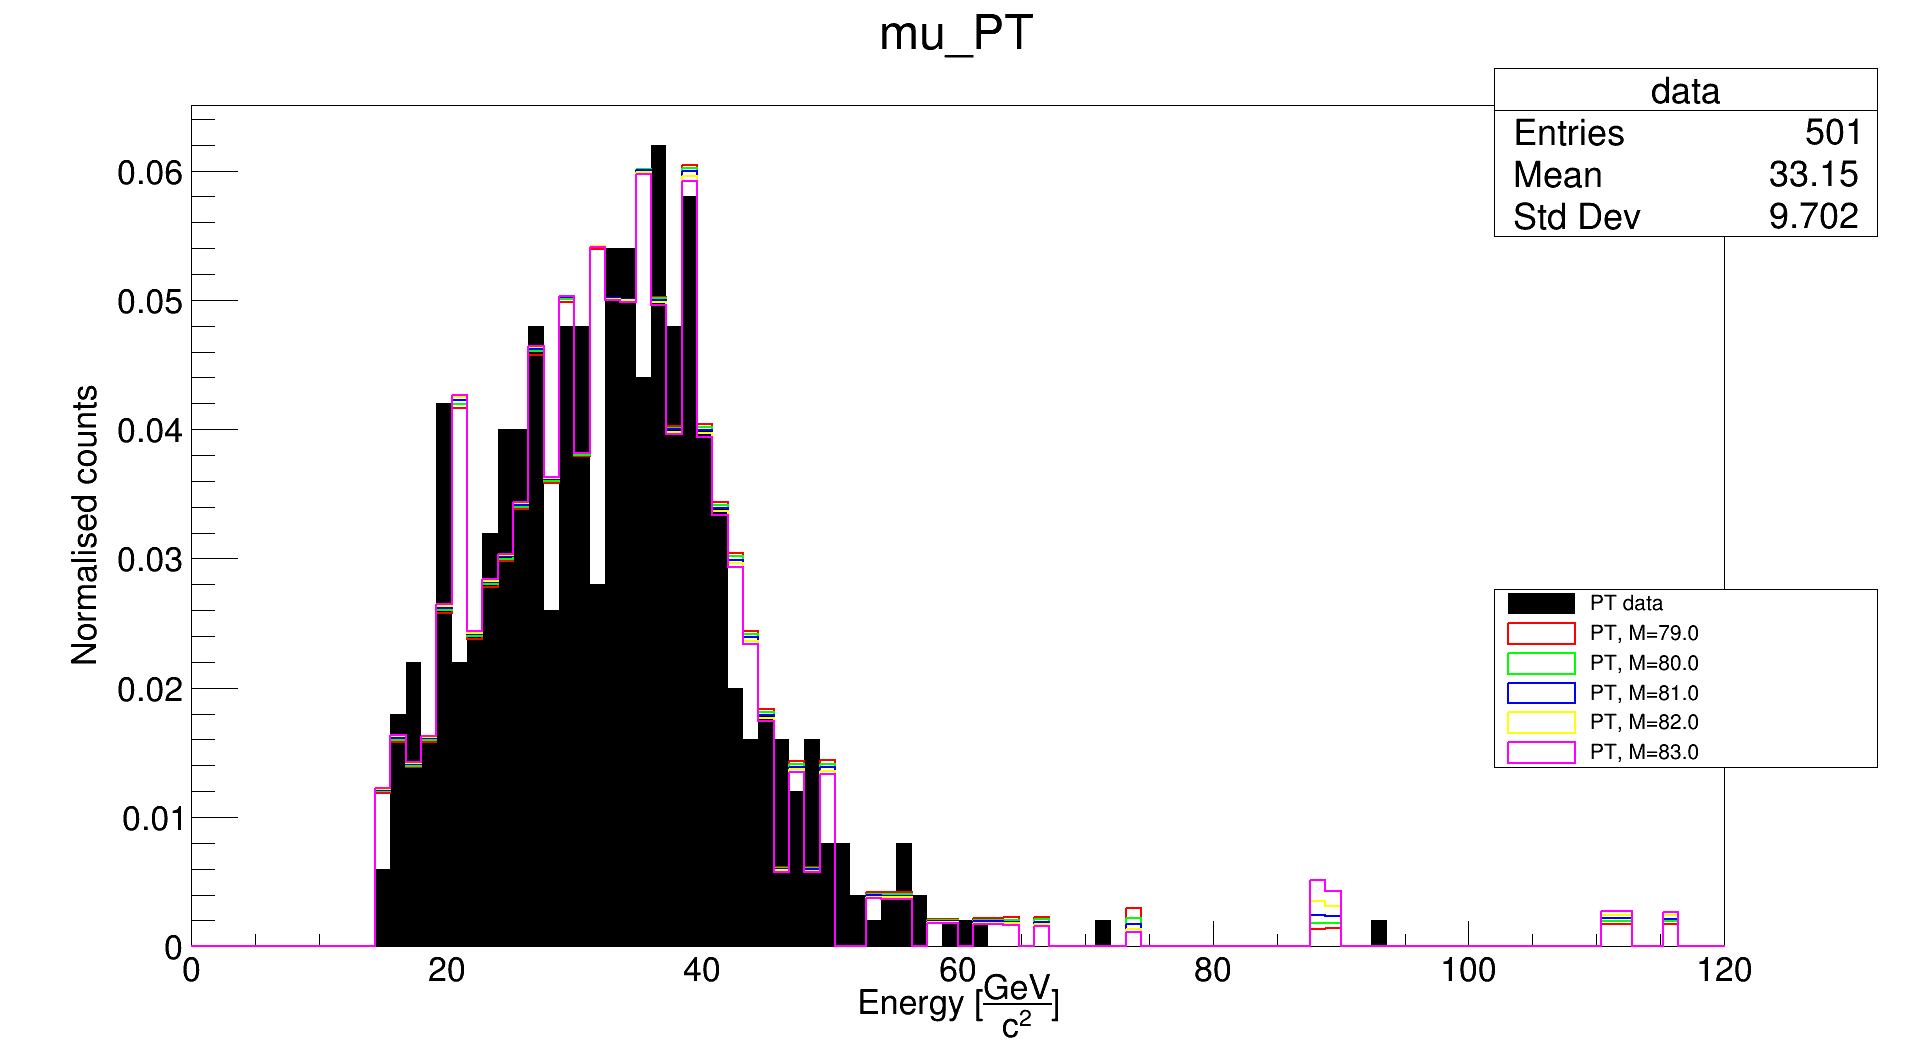
\includegraphics[width=\columnwidth]{/home/physics/phuxdp/Desktop/WBosonProject/templates/plots/muPT_80.36010913_2.07041274_between_79_and_83.png}
		\caption{\small Number of data points used: 1000, mean expected W mass: 80.36010913 [GeV/c^2], mean hypothesis masses: [79. 80. 81. 82. 83.] [GeV/c^2], mass width: 2.07041274 [GeV/c^2], chi_square value of hypothesis fit: 0.00029114840214308296 from /home/physics/phuxdp/Desktop/WBosonProject/templates/plots/muPT_80.36010913_2.07041274_between_79_and_83.png }
		\label{fig: fig_0}
	\end{figure}

\end{document}